\section{Analisis Hasil Pengujian}

\subsection{Siklus Penjualan Tiket}

Kedua skenario pengujian ini memiliki siklus permintaan yang berbeda. Siklus dalam hal ini berarti fase ketika sistem memiliki pola permintaan yang berbeda. Contoh pada skenario beban berkelanjutan diambil dari pengujian f1t2, sedangkan contoh pada skenario perebutan tiket diambil dari pengujian f1t4. Siklus/pola ini juga terjadi pada skenario serupa ketika proses penjualan berjalan dengan lancar.

\subsubsection{Skenario Beban Berkelanjutan}

\begin{figure}[htbp]
    \centering
    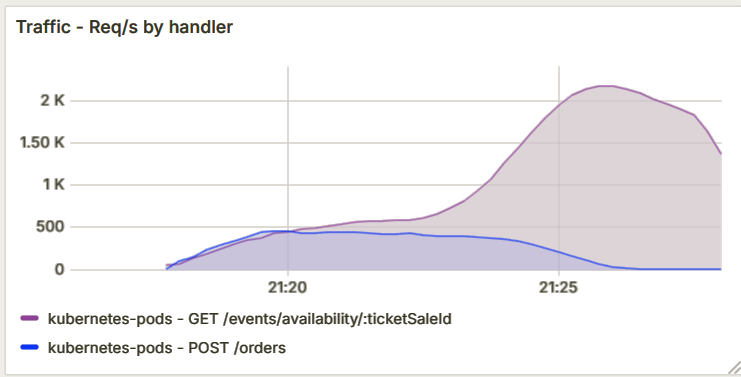
\includegraphics[width=0.6\textwidth]{resources/chapter-4/pattern-stress-traffic.png}
    \caption{Pola Permintaan pada Beban Berkelanjutan}
    \label{fig:pattern-stress-traffic}
\end{figure}

Pada skenario ini, sistem memiliki ketersediaan tiket yang banyak sehingga penjualan tiket yang berhasil berjalan cukup lama. Setelah tiket habis terjual, jumlah permintaan ketersediaan tiket jauh meningkat karena penguji mencoba mencari tiket dari berbagai area dengan lebih banyak.

\begin{figure}[htbp]
    \centering
    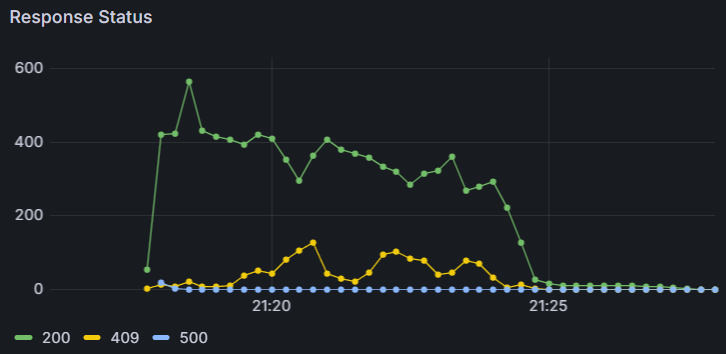
\includegraphics[width=0.6\textwidth]{resources/chapter-4/pattern-stress-order.png}
    \caption{Status Respons pada Beban Berkelanjutan}
    \label{fig:pattern-stress-order}
\end{figure}


Status respons pemesanan tiket menunjukkan bahwa terjadi konflik (kode 409) selama pemrosesan pesanan sebanyak 3-10\% dari respons secara keseluruhan.

\pagebreak

\subsubsection{Skenario Perebutan Tiket}

\begin{figure}[htbp]
    \centering
    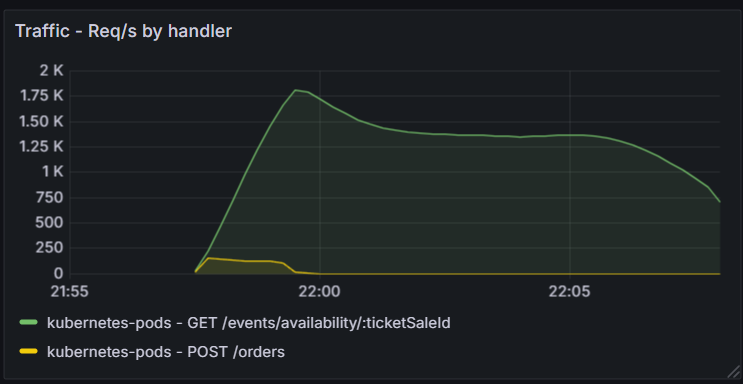
\includegraphics[width=0.6\textwidth]{resources/chapter-4/pattern-sim-traffic.png}
    \caption{Pola Permintaan pada Perebutan Tiket}
    \label{fig:pattern-sim-traffic}
\end{figure}

Pada skenario ini, jumlah permintaan ketersediaan jauh lebih banyak dibandingkan permintaan pemesanan tiket. Hal ini wajar karena terdapat lebih banyak peminat dibandingkan dengan tiket yang tersedia. Berdasarkan grafik di atas, tiket habis terjual dalam kurang lebih 2 menit penjualan.

\begin{figure}[htbp]
    \centering
    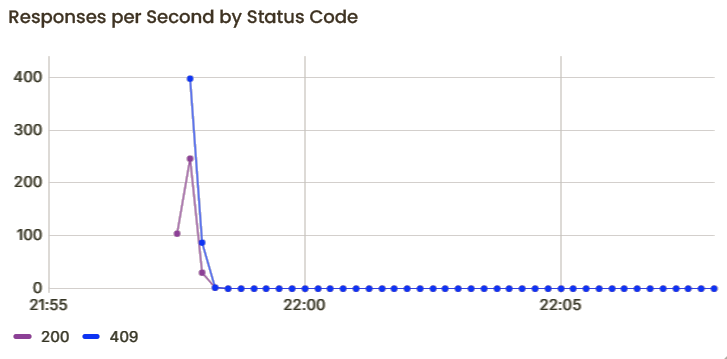
\includegraphics[width=0.6\textwidth]{resources/chapter-4/pattern-sim-order.png}
    \caption{Status Respons pada Perebutan Tiket}
    \label{fig:pattern-sim-order}
\end{figure}

Status respons pemesanan tiket menunjukkan bahwa terjadi konflik (kode 409) yang cukup banyak bahkan sejak proses penjualan dimulai. Pengguna yang baru masuk setelahnya pada akhirnya akan gagal memperoleh tiket, sebagaimana digambarkan pada keadaan akhir penguji pada gambar berikut.

\begin{figure}[htbp]
    \centering
    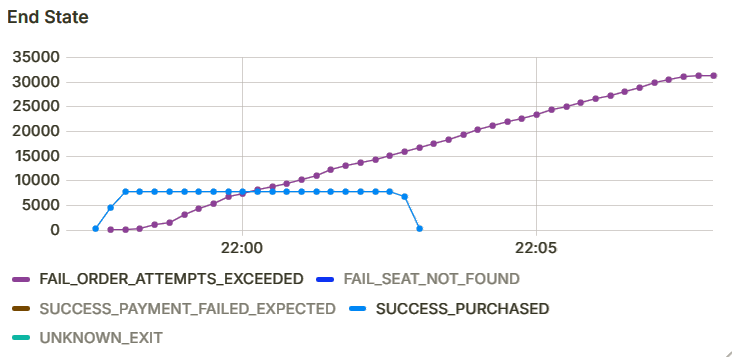
\includegraphics[width=0.6\textwidth]{resources/chapter-4/pattern-sim-k6.png}
    \caption{Keadaan Akhir Penguji pada Perebutan Tiket}
    \label{fig:pattern-sim-k6}
\end{figure}


\subsection{Kinerja Selama Pengujian}

Secara garis besar, varian PostgreSQL mampu menangani beban yang diberikan dengan sangat baik. Varian CitusData masih memiliki kinerja yang baik, meski memiliki latensi yang lebih tinggi dibandingkan dengan PostgreSQL. YugabyteDB mengalami lebih banyak kegagalan dan kinerja yang buruk sehingga tidak dapat menyelesaikan proses penjualan dengan baik. Sampel pengujian yang dipilih pada adalah skenario stress-2 tanpa pengendalian aliran. Skenario ini merupakan skenario pengujian dengan kinerja YugabyteDB yang dapat diterima dan mampu menyelesaikan proses penjualan. Dengan beban yang lebih tinggi, YugabyteDB mengalami banyak kegagalan. Pembahasan lebih lanjut hasil pelaksanaan setiap pengujian dibahas pada lampiran \ref{apx:test-run-performance}.

\begin{table}[h]
    \centering
    \caption{Gambaran Kinerja Permosesan Pesanan}
    \begin{tabular}{|l|l|l|l|}
        \hline
        \textbf{Metrik} & \textbf{PostgreSQL} & \textbf{CitusData} & \textbf{YugabyteDB} \\
        \hline
        \textit{Throughput} Maksimum & 466 rps & 410 rps & 216 rps \\
        \hline
        Penggunaan CPU (Puncak) & 8 vCPU & 10 vCPU & 19 vCPU \\
        \hline
        Penggunaan Memori (Puncak) & 3.4 GB & 5 GB & 36 GB \\
        \hline
        Latensi Pemrosesan (P50) & 192-382 ms & 496-650 ms & 854-10000 ms \\
        \hline
    \end{tabular}
\end{table}

Latensi dan \textit{throughput} pemrosesan diukur dari sisi Ticket Server, bukan dari level basis data. Latensi pemrosesan yang diambil merupakan latensi terbaik saat beban sudah cukup tinggi dan laju pemrosesan mulai stabil. Penggunaan CPU dan penggunaan memori merupakan agregat puncak jumlah penggunaan sumber daya setiap instans basis data yang berkaitan. Apabila terdapat dua nilai maksimal \textit{throughput} yang mendekati, nilai yang dipilih adalah nilai yang memiliki rasio sukses (respons 200) paling tinggi.

Berdasarkan tabel di atas, PostgreSQL unggul dari segala aspek, mulai dari laju pemrosesan, penggunaan sumber daya, serta latensi. CitusData memiliki laju pemrosesan yang mendekati PostgreSQL dengan latensi 2x lebih lambat dan penggunaan sumber daya yang sedikit lebih tinggi. Di sisi lain, YugabyteDB memiliki laju pemrosesan kurang dari setengah PostgreSQL dengan latensi setidaknya 4x lebih lambat, penggunaan CPU 2.4x lebih banyak, dan penggunaan memori 10x lebih banyak.

\subsection{Kinerja Basis Data Terdistribusi}



Bandingkan kinerja setiap basis data. highlight how optimized postgres

postgres, citus, yugabyte.

tabel kueri juga -> jelasin efisiensi kueri tiap varian.

mention juga bahwa selama pengujian ternyata emang banyak banget kueri baca dan bebannya ga bisa dibiarin.

jelaskan citus yugabyte struggle juga buat handle kueri baca.

\subsubsection{Mengapa CitusData tidak perform}

beban pada koordinator. mostly read.

ambil hasil referensi TPC-C dan github issue.

jelaskan bagian citusdata yg bakal lebih optimal kalau pake stored procedure.

\subsubsection{Mengapa YugabyteDB tidak perform}

limit koneksi, butuh sumberdaya yang lebih besar. tidak cocok untuk high concurrent transaction. banyak terjadi kegagalan transaksi jadinya diretry.

ambil hasil referensi pengujian juga (pokoknya artikel yg bandingin raw performance)

\subsection{Pengoptimalan Kueri Baca}

buktikan kalau kueri ini banyak banget dipanggil -> pakai grafik/ data dari grafana.  

refer ke redis. pakai data pengujian fc postgres (jgn nofc). 

apakah hasilnya oke?

\subsection{Integritas Tiket selama Perebutan Tiket}

Apakah terjadi perbedaan data ketersediaan, dropper availability?

Apakah terjadi double booking?

\subsection{Penggunaan Pengendalian Aliran}

Jelasin berapa banyak request yg ditolak (respons 409). Gbs response based on code? atau apa gitu bandingin latensinya fak.

Dampaknya gimana (blm tau).

\subsection{Keterbatasan Pengujian}

List keterbatasan apa aja yang ada selama pengujian/ analisis yang mengakibatkan hasil kinerja bisa jauh berbeda.

jumlah virtual user yang dikit.

harusnya ngikutin distribusi sesuai gambar drpd load test

pakai resource lebih banyak agar lebih fair ke yugabytedb.

pisah penanganan kueri baca tulis agar resource usage utk tiap operasi bisa dibedain -> dampaknya lebih bisa diukur. kalau skrg banyak noise.
